% The end to end process: second chapter.

\chapter{End to End: From Source to eReader}

We'll start with the end-to-end process for making a book you can read
on your eReader device. Checking that you can do this, change the title,
add or remove chapters, and see the changes you've made reflected on your 
eReader, will hopefully be the best encouragement to work through more
of this book, focusing on the topics that are most useful for your own book.

\begin{figure}
\begin{center}
  
\includegraphics[width=1.2\linewidth]{images/pipeline.png}
 \vspace{0.2cm}
\caption{Steps in the pipeline for shipping this eBook}
\end{center}
\label{fig:pipeline}
\vspace{0.4cm}
\end{figure}

The basic outline of the process is shown in Figure \ref{fig:pipeline}.
The rest of this chapter serves to describe the steps in more detail.

The descriptions of commands here will be relatively high-level ---
we'll say things ``install git and run git clone'', rather than giving
details on how to do this on various operating systems. This is for
three reasons. The first is that it's easier to write instructions
this way. The second is that very specific instructions of which web
addresses to visit and which buttons to click on can go stale very
quickly. The third is that this book does assume that the reader has
some experience with and / or tolerance for figuring out a certain
amount of installation and troubleshooting on computers. If not, try one of the
more constrained off-the-shelf tools that are easier to get started with
than \latex. 

%%
\section{Install Dependencies}

Typically when you want to use a new piece of software, it has
dependencies --- other libraries and packages it needs for some of its
functionality. For end-user applications, these are usually bundled
together so that everything works `out of the box'. For programming
tools, there's normally some system to check which dependencies you
already have, and to install only the new ones that you need. How this
works depends partly on what platform you're using. Here we'll just list
the dependencies you'll need to find and install.

These include:

\begin{itemize}
\item A \latex system, including a program called \smalltt{make4ht} or the older \smalltt{htlatex}.
  This is crucial for making HTML output, as described in Section
  \ref{sec:html2epub}.
\item Some eBook converter software. The one recommended below is
  \smalltt{ebook-convert}, from Calibre (see
  {\small \url{https://manual.calibre-eBook.com/ebook-convert.html}}, or just
  search the web).
\item Some eReader or previewer software, such as a Kindle device or
  app, or another eBook app such as Calibre (see above). You'll want
  this for seeing how your book looks `for real' (though of course,
  not all eBook apps look exactly alike.
\item (Recommended) A shell program that runs bash scripts so that you
  can run the \smalltt{build.sh} command. If you don't already have a
  terminal where you can run bash or a close equivalent, it's probably
  worth installing and using, and if that instruction sounds
  difficult, the rest of the process may be hard.
\end{itemize}

Every modern operating system --- basically Windows, Linux, MacOS, and
similar variants --- has a variety of package installation tools.
Some of the above can be done at the command-line, sometimes it's
easier to download and install something directly from a provider's
website.

The best place to keep links to such dependencies is the 
github project wiki at {\small \url{https://github.com/dwiddows/ebookbook/wiki}}.

%%
\section{Access and Build the \latex Source}

Next, you'll want to get a copy of the source code for this
book. (We won't split hairs about whether \latex sources count as
`code'. It gives instructions to machines, it's easy to make mistakes
that show up as error messages, and it's reviewed and stored in source
control --- so it's like code in these practical senses.)

If you already have \smalltt{git} installed, this will be something
like running \smalltt{git clone
  https://github.com/dwiddows/ebookbook.git} at a command prompt, or
downloading the code using some visual client software. 

List the contents of this directory and check that you can see the
files \smalltt{ebookbook.tex} and \smalltt{build.sh}. The first of these
is the main \tex document that lays out how to combine the other files
into an eBook.  The second is a build script --- on platforms with
bash or a compatible shell installed, you should be able to run just
\smalltt{./build.sh} and get most of the book built using one
command. Or at least, to begin with, you should get error messages
telling you if anything is missing and needs to be installed. If you're not
running a compatible shell, the \smalltt{build.sh} at least lists
the commands you'll need to run some other way.

So the next step is to run \smalltt{./build.sh} and ideally it should
typeset a copy of this book. If the \smalltt{ebook-convert} command is
available it should even make the eBook files described in the next
section.

If this doesn't work, you may need to find and install some
\smalltt{pdflatex} and most importantly \smalltt{make4ht} or
\smalltt{htlatex} programs that work on your machine. (See the
Dependencies section above.)

%%
\section{From HTML to ePub ... or Mobi}
\label{sec:html2epub}

The most important output from the previous step is a file called
\smalltt{ebookbook.html}.  This is formatted for display as a webpage
in a browser. This is different from the more common use of \tex to
make documents such as academic papers, which are nowadays normally
created as PDF files. An HTML file is a collection of content (for
example, words and images to display), and typesetting suggestions
(for example, make this text a heading, and make this image 40\% of
the screen width). This is different from a PDF file, which has
precise instructions about how big to make each character and which
page to put it on. So it makes sense that HTML is more like an eBook:
instead of saying what text will appear on which page, it gives
directives about what text should be bigger and smaller, and this
combines with the user's device settings to decide which page it
should appear on.

So the \smalltt{ebookbook.html} file (rather than the corresponding
PDF file or any other page-layout format) will be used to
create your eBook format. 

You can turn your HTML file form a webpage into an eBook by installing
and using a converter such as Calibre \smalltt{ebook-convert} or
Amazon's {\em Kindle Previewer} tool.
There are a range of such converters and previewers, targetting a
variety of formats, and this is another place where the complexity of
electronic publication is obvious. Like saving an image as a
\smalltt{.jpg}, \smalltt{.gif} or \smalltt{.png}, you'll need to select a
format to convert to, and options include:

\begin{itemize}
  \item \smalltt{epub} is a cross-platform format that it supposed to
    be used for any electronic book.
  \item \smalltt{mobi} is an old Amazon Kindle format --- and it
    happens to be the one you can use for e-mailing files to your Kindle.
\end{itemize}

The \smalltt{build.sh} script that comes with this book uses
\smalltt{ebook-convert} and creates both \smalltt{epub} and
\smalltt{mobi} files as output. This also takes command-line
arguments so that you can specify metadata like the author name
and cover image:

{\flushleft \quad \smalltt{ebook-convert ebookbook.html ebookbook.epub --cover images/cover.jpg --authors "YOUR NAME" --language English}}

%%
\section{Previewing Your Book on an eReader}

Hopefully by now you have an eBook. Or at least, a file called something like
\smalltt{ebookbook.epub}. So how do you {\em read} your book?

For this you'll need an eReader --- perhaps an app on your computer or phone,
or an eReader device such as a Kindle.

Assuming that most of your writing will be on a computer, that's
probably the first place you'll want to see your work. For example, I
usually open the Calibre app and load the epub file, or do both at
once with the command \smalltt{calibre ebookbook.epub}. Once the book is imported and loaded, this gives 
the satisfying result shown in Figure \ref{fig:calibre_screenshot}.

\begin{figure}
  \begin{center}
  \vspace{0.2cm}
\fbox{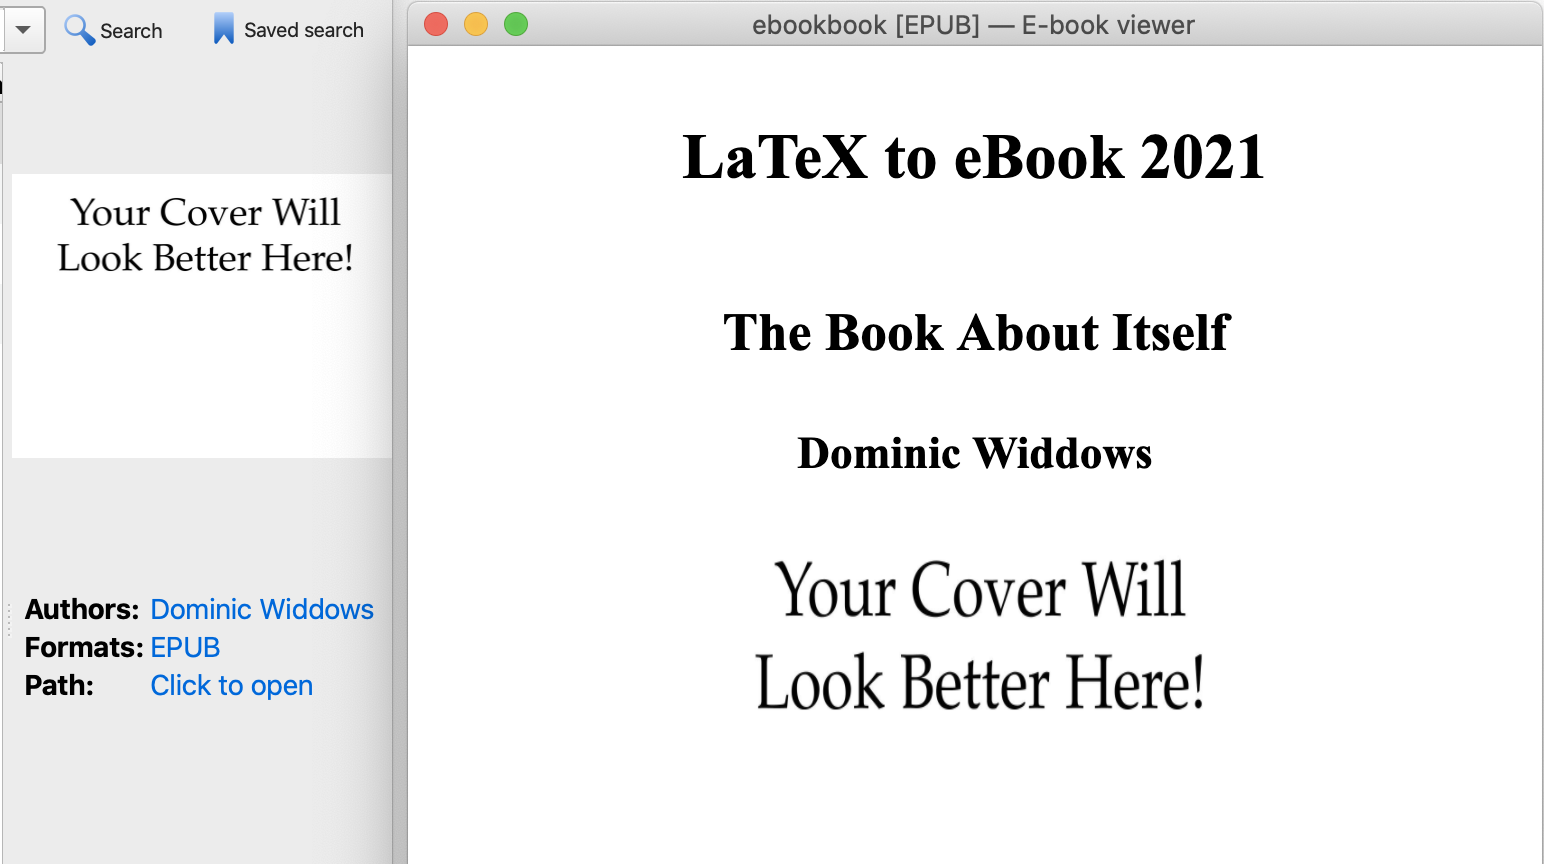
\includegraphics[width=\linewidth]{images/calibre_screenshot.png}}
\caption{Book thumbnail image and cover page in the Calibre eReader}
\vspace{0.4cm}
\label{fig:calibre_screenshot}
\end{center}
\end{figure}

To view on an eReader device or phone, you often have to send it to
the device or load it on in some way --- again, there are a range of
methods. For Amazon Kindles, you need to find / set up an email address for the
device itself, and send the book to that email address. As an extra
complexity, this method only works using the older \smalltt{mobi}
files.  Also Kindle preloads like this do not (at the moment)
display the cover page of the book in your library or menu page,
because Amazon retrieves this information for {\em published} books
from elsewhere. So the preview in the library view is somewhat
disappointing, but it works (Figure \ref{fig:kindle_screenshot}).

\begin{figure}
  \begin{center}
  \vspace{0.2cm}
  \fbox{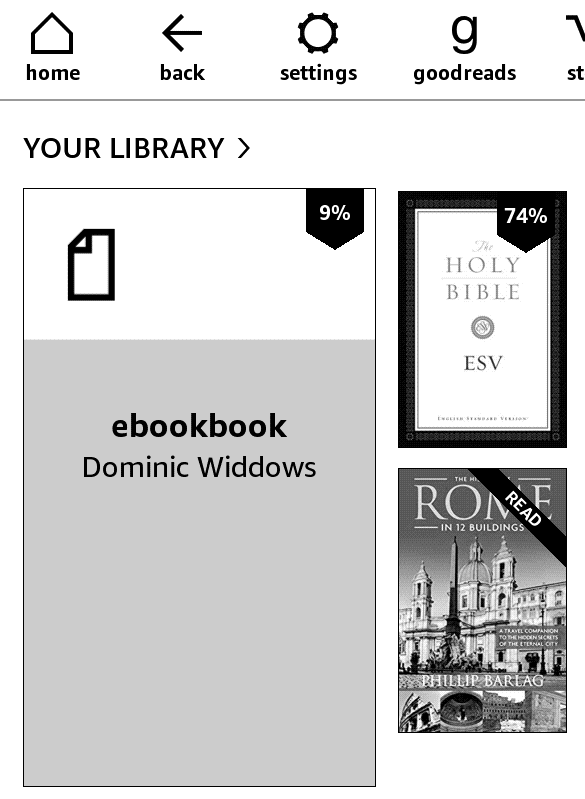
\includegraphics[width=0.6\linewidth]{images/kindle_screenshot.png}}
  \caption{Book thumbnail image loaded onto a Kindle}
  \label{fig:kindle_screenshot}
  \vspace{0.4cm}
 \end{center}
\end{figure}

%%
\section{Make it Your Own!}

Hopefully by now you're at the point where there is an epub file that you can easily read on some eReader device or app. 

The next thing you should do is {\em change something}. Change the title in the \smalltt{cover\_page.tex} file from `\latex to eBook 2021'
to whatever title you want. Rerun the steps above and hopefully you'll see exactly what you intended: a copy of the eBook, but with
your title instead.

At this point you're off to the races. That doesn't mean that it's all plain sailing from here, there will doubtless be glitches and hurdles along the way.
But the main thing is that you have a template, examples of several \latex constructs that work with eBooks, and you're able to start turning this
into your own book. You may want to save your work separately at this point, call the project something else, and if you use source control,
start checking in your work in some way that makes it clear that it's a new project, rather than a work-in-progress on the old project that's intended to be
merged back in at some point.

Experiment with removing directives to \smalltt{\textbackslash input} different chapters, and watch the book get shorter. Try changing image files to some other graphic
and make sure they change appropriately. And try editing the AUTHOR in the \smalltt{build.sh} file and make sure the right name shows up when the book is viewed in an eReader.

If this works, you can be pretty confident that your book is on the right track. You'll be able to organize the content into \tex files, image files, etc., and create an eBook!


%%%
\section{Publication}

Nearly all of this book is about how to create and preview eBook files, and this is like a software development process
--- you should be able to run the pipeline over and over again and keep testing that the change you made had the desired effect.

Publishing and marketing your book is a different story: you'll basically be using an online browser app, signing up for accounts, uploading files, filling in forms,
you'll eventually click "submit", and hopefully see your book available for download / purchase after a short while (like a couple of days).

This is exactly the process I am going through right now with Amazon Kindle. So far it's straightforward enough form-filling. Hopefully it's that easy throughout.
If you bought this book in the Kindle store and can read this as a result, please assume it worked. And if I could do this, you can too!





